\textbf{符号位的处理:一般来讲,符号位的处理有以下两种方式:}

\textbf{1.无符号数的表示}

无符号数指整个机器字长的全部二进制位均为数值位,没有符号位,相当于数的绝对值。若机器字长为8位,则数的表示范围为0~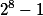
\includegraphics[width=0.44792in,height=0.16667in]{texmath/b4598028-1},即0~255。

\textbf{2.有符号数的表示}

有符号数需要将其符号数字化,即``0''表示正号,``1''表示负号。下面介绍3种有符号数的表示方法:原码、补码、反码。\\

友情提示:不少考生觉得运算器比较复杂难懂,很大程度上是因为分段函数,例如:

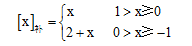
\includegraphics[width=2.00000in,height=0.47917in]{png-jpeg-pics/74926997B7159E2348695202D4DC1894.png}

\textbf{{计算真值的原码、补码、反码、移码更简单的方法,根本不用管这个分段函数,就是用下面3句话解决问题,简单易懂。}}

\textbf{第1句:}3种机器数的最高位均为符号位。符号位和数值部分之间可用``.''(对于小数)或``,''(对于整数)隔开。

\textbf{第2句:}当真值为正数时,原码、补码和反码的表示形式均相同,即符号位用``0''表示,数值部分与真值相同。

\textbf{第3句:}当真值为负数时,原码、补码和反码的表示形式不同,但其符号位都用``1''表示,而数值部分有这样的关系,即补码是原码的``每位求反加1'',反码是原码的``每位求反''。需要注意的是,上面所谓的``每位求反''均不包括符号位,只是对数值部分进行求反,且原码除了符号位为``1'',数值部分仍然与真值相同。
